% vim:ft=tex:
%
\documentclass{standalone}
\usepackage{tikz}
\usetikzlibrary{decorations.text,patterns,shapes}
\usepackage{xcolor}
\colorlet{robotino}{green!30!black}
\colorlet{bounding-box}{blue!30!black}
\colorlet{gripper-reach}{red!50!black}
\begin{document}
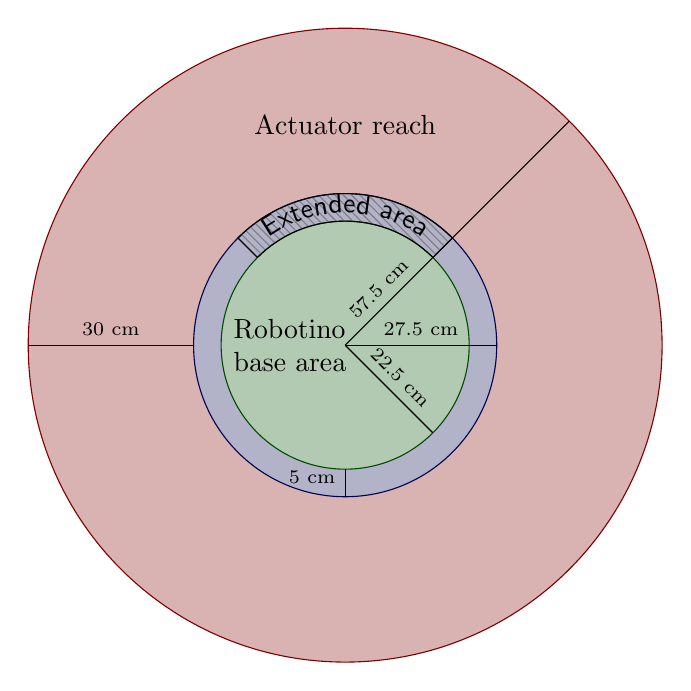
\begin{tikzpicture}
	\begin{scope}[scale=0.7]
	%	\node (A) [cylinder, shape border rotate=90, draw,minimum height=7cm,minimum width=5.5cm, fill=bounding-box!30!white] at (-10,0) {};
	%	\node (B) [cylinder, shape border rotate=90, draw,minimum height=3cm,minimum width=4.5cm, fill=robotino!30!white,anchor=south] at (A.south)
%{};
%\draw [<->] ([yshift=0.4cm]A.before top) -- ([yshift=0.4cm]A.after top) node [midway, above,fill=white] {55 cm};
%\draw [<->] ([xshift=-0.2cm]A.before top) -- ([xshift=-0.2cm]A.after bottom) node [midway, left,fill=white] {180 cm} node[pos=0.2,sloped,fill=white] {$\ldots$};
	\draw[gripper-reach,fill=gripper-reach!30!white] (0,0) circle (5.75cm);
	\draw[bounding-box,fill=bounding-box!30!white] (0,0) circle (2.75cm);
	\draw[robotino,fill=robotino!30!white] (0,0) circle (2.25cm);
	\draw (0,0) --  (-45:2.25cm) node [midway,above,sloped]{\scriptsize 22.5 cm};
	\draw (0,0) --  (0:2.75cm) node [pos=0.5,above,sloped]{\scriptsize 27.5 cm};
	\draw (0,0) --  (45:5.75cm) node [pos=0.2,above,sloped]{\scriptsize 57.5 cm};
	\draw (0,-2.25) --  (0,-2.75) node [pos=0.3,left]{\scriptsize 5 cm};
	\draw (-2.75,0) --  (-5.75, 0) node [pos=0.5,above]{\scriptsize 30 cm};
	\draw[pattern=north west lines, pattern color=black!50!white] ([shift=(45:2.25cm)]0,0) arc (45:135:2.25cm) --
		([shift=(135:2.75cm)]0,0) arc (135:45:2.75cm) -- cycle;
	\path[postaction={decorate,decoration={text along path,text align=center,text={|\sffamily|Extended area}}}] (-2.4,0) arc[
        start angle=180,
        end angle=0,
        x radius=2.4cm,
        y radius =2.4cm
    ]
		;
	\node[anchor=west,align=left] at (-2.2,0) {Robotino\\base area};
	\node at (0,4) {Actuator reach};
\end{scope}
\end{tikzpicture}
\end{document}
